\documentclass{article}

\usepackage[english]{babel}
\usepackage[utf8]{inputenc}
\usepackage[T1]{fontenc}
\usepackage{lmodern}
\usepackage{amsmath}
\usepackage{graphicx}
\usepackage{hyperref}
\hypersetup{colorlinks,citecolor=black,linkcolor=blue}

\graphicspath{{New/}}
\let\biblio\bibliography
\let\bibsty\bibliographystyle
\renewcommand{\bibliography}[1]{\expandafter\biblio{New/#1}}
\renewcommand{\bibliographystyle}[1]{\expandafter\bibsty{New/#1}}

% =============================================================================

\title{Latexpand \& Latexdiff}
\author{Juan C. Garnica A.}
\date{April 2023}

\begin{document}


\maketitle

\section{Introduction}
We can cite references \cite{QFT-RG-notes}\footnote{Notice that the numbering will not be fixed in this pdf but it will be consistent within each of the latexpanded versions of the old and new projects.}

\section{A modified section}

This was modified to include Figure \ref{fig::1} and Eq. \eqref{eq::1}.

\vspace{0.5cm}
\begin{figure}[h]
\centering
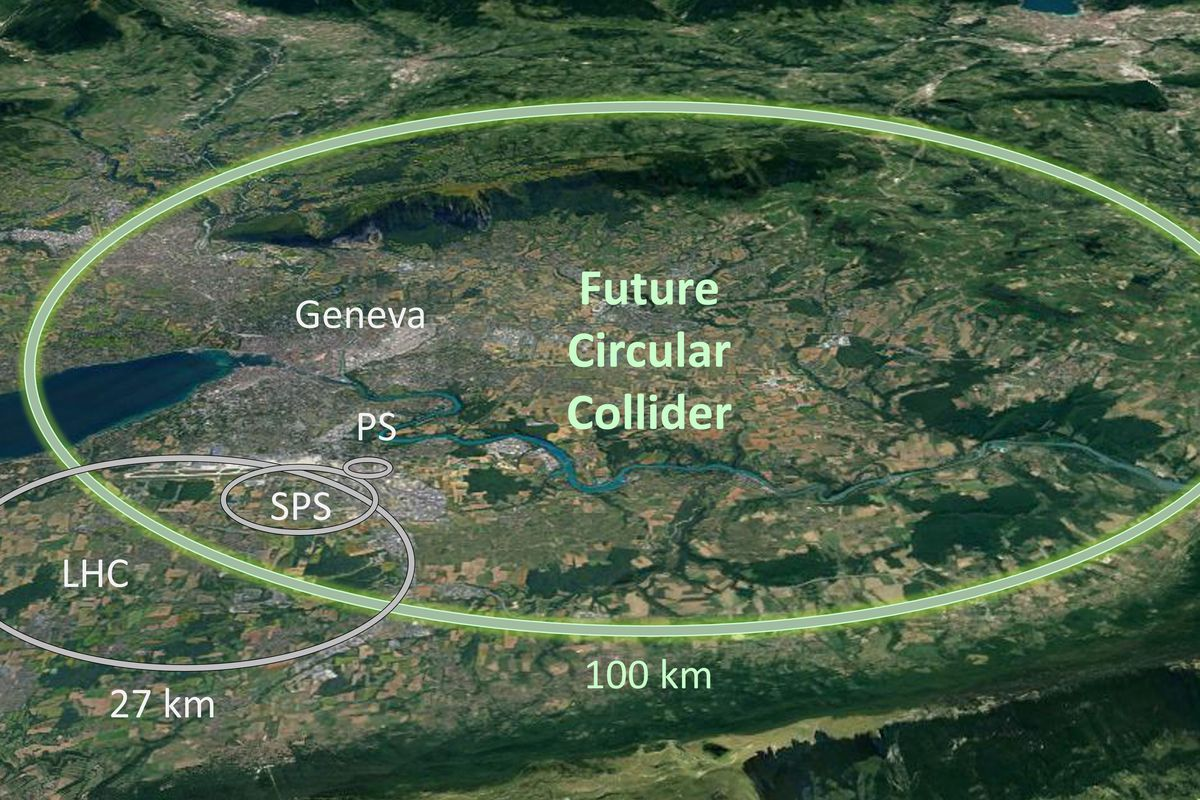
\includegraphics[width=0.4\textwidth]{Images/fcc.jpg}
\caption{\label{fig:frog}Coming soon, 2040.}
\label{fig::1}
\end{figure}

\begin{gather}
a^2+b^2=c^2
\label{eq::1}
\end{gather}


\newpage
\section{This section has been added}
zzz

\vspace{1cm}
\bibliographystyle{hep}
\bibliography{Biblio}

\end{document}
